\documentclass[12pt]{article}

\usepackage{times,mathptmx}
\usepackage[pdftex]{graphicx}
\usepackage{pdflscape}

\usepackage{subcaption}
\usepackage{graphicx}
\usepackage{float}
\usepackage[section]{placeins}
\usepackage{fancyhdr}
\usepackage{enumitem}

\usepackage{tocloft}
\usepackage[nottoc,notlof,notlot]{tocbibind} % Put the bibliography and index in the ToC

\pagestyle{fancy}
\rhead{}
\lhead{}
\chead{}
\cfoot{Page \thepage}
%\renewcommand{\headrulewidth}{0.4pt}
\renewcommand{\footrulewidth}{0.4pt}

\usepackage{color}
\usepackage{amsmath}
\usepackage{multirow}
\definecolor{linknavy}{rgb}{0,0,0.50196}
\definecolor{linkred}{rgb}{1,0,0}
\definecolor{linkblue}{rgb}{0,0,1}

\usepackage{xr-hyper}
\usepackage[pdftex,
        colorlinks=true,
        urlcolor=linkblue,     % \href{...}{...} external (URL)
        citecolor=linkred,     % citation number colors
        linkcolor=linknavy,    % \ref{...} and \pageref{...}
        pdfproducer={pdflatex},
        pagebackref,
        pdfpagemode=UseNone,
        bookmarksopen=true,
        plainpages=false,
        verbose]{hyperref}

\setlength{\textwidth}{6.5in}
\setlength{\textheight}{9.0in}
\setlength{\topmargin}{0.in}
\setlength{\headheight}{0.in}
\setlength{\headsep}{0.1in}
\setlength{\parindent}{0.25in}
\setlength{\oddsidemargin}{0.0in}
\setlength{\evensidemargin}{0.0in}




\begin{document}

\bibliographystyle{unsrt}
\thispagestyle{empty}


\vspace*{0.75in}

\begin{center}
\begin{Large}
{\bf Guidelines for Participation in the MaCFP-3 Workshop} \\
\end{Large}
\begin{large}
October 2023\\
Tsukuba, Japan
\end{large}
\hspace{1in} \\
\end{center}


\begin{figure}[h]
  \centering
  \includegraphics[width=6in]{../MaCFP_Logo.pdf}
  \label{Cover_Image}
\end{figure}

\vfill

\begin{minipage}{0.25\textwidth}
\begin{figure}[H]
\includegraphics[width=1.8in]{../IAFSSLogo.pdf}
\end{figure}
\end{minipage} \hfill
\begin{minipage}{0.75\textwidth}
\begin{flushright}
\begin{small}
{\bf The MaCFP Condensed Phase Working Group Organizing Committee:} \\
Benjamin Batiot (University of Poitiers, France) \\
Morgan Bruns (Virginia Military Institute, USA) \\
Simo Hostikka (Aalto University, Finland) \\
Isaac Leventon (National Institute of Standards and Technology, USA) \\
Yuji Nakamura (Toyohashi University of Technology, Japan) \\
Pedro Reszka (Universidad Adolfo Ibáñez, Chile) \\
Thomas Rogaume (University of Poitiers, France) \\
Stanislav Stoliarov (University of Maryland, USA)
\end{small}
\end{flushright}
\end{minipage}

\newpage
\thispagestyle{empty}
\tableofcontents

%\mainmatter
\pagestyle{empty}
\newpage
\section{Background}
\subsection{MaCFP Working Group Motivation}
The general objective of the MaCFP Working Group is to establish a structured effort in the fire research community to make significant and systematic progress in fire modeling, based on a fundamental understanding of fire phenomena. The strategy is based on the study of elementary academic problems and a gradual move towards complexity and realism by following a building block approach to model development. This is to be achieved as a joint effort between experimentalists and modelers, identifying key research topics of interest as well as knowledge gaps, and thereby establishing a common framework for fire modeling research. The MaCFP Working Group is intended as an open, community-wide, international collaboration between fire scientists. It is also intended to be a regular series of workshops.

The specific objectives of the MaCFP Working Group are to: 
\begin{itemize}[noitemsep]
 \item Develop a digital archive of well-documented fire experiments that can be used as targets for CFD model validation; 
 \item Develop a digital archive of well-documented CFD-based numerical simulations corresponding to the selected target experiments; 
 \item Develop protocols for detailed comparisons between computational results and experimental measurements; 
 \item Identify key research topics and knowledge gaps in computational and experimental fire research; 
 \item Develop best practices in both computational and experimental fire research (including quality control and quantification of uncertainties); 
 \item Establish a network between fire researchers and provide a community-wide forum for discussion and exchange of information.	
\end{itemize}

\subsection{The Gas Phase Subgroup}
The initial list of target experiments identified by the MaCFP Working Group includes five categories:
\begin{itemize}[noitemsep]
 \item Category 1: Turbulent buoyant plumes;
 \item Category 2: Turbulent pool fires with gaseous fuel;
 \item Category 3: Turbulent pool fires with liquid fuel;
 \item Category 4: Turbulent wall fires;
 \item Category 5: Flame extinction;
 \item Category 6: Fire growth.
\end{itemize}
These target experiments correspond to basic configurations (building blocks) with carefully-controlled conditions and quality instrumentation and diagnostics. They also correspond to available open databases. This list will be enhanced as the MaCFP Working Group makes progress and moves towards greater complexity and realism. At MaCFP-3, a new category will be presented and studied: Category 6, Fire Growth

\subsection{The Condensed Phase Subgroup}
Historically, the fire modeling community has self-organized into two distinct groups: a first group that studies combustion and heat transfer in the gas phase, and a second group that studies thermal degradation and pyrolysis in the condensed phase. The early discussions of the MaCFP Working Group have focused on gas phase phenomena, but with the understanding that quantitatively predicting flame spread and fire growth requires modeling of coupled gas phase and condensed phase processes. Following discussions that took place in April 2016, it was proposed that the MaCFP Working Group be expanded to include a subgroup dedicated to the predictive modeling of condensed phase phenomena. A committee was formed to produce a white paper and organize a planning meeting during the first MaCFP workshop conducted in Lund, SE at the 2017 IAFSS meeting~\cite{brown2018proceedings}. 

\subsubsection{MaCFP-1: Lund, Sweden (2017)}
The purpose of the Condensed Phase Phenomena subgroup is to facilitate data sharing and model development to improve computational predictions of thermal degradation and pyrolysis in fire scenarios. At MaCFP-1, a review was  presented of the challenges associated with pyrolysis measurements and modeling for fire applications. Review topics included: identifying experimental apparatus, datasets, and associated analysis tools needed to calibrate the material properties used in computational pyrolysis models (i.e., model inputs); providing accurate descriptions of the condensed- and gas-phase processes occurring at the solid/gas interface, which control ignition and flame spread; discussion of the relevant complexity needed to describe condensed-phase material decomposition and the capabilities of various numerical tools to capture these phenomena; and the need to validate these models to predict material burning behavior across a range of scales. Open discussion between participants of this meeting provided critical input from the fire research community regarding test methods of interest and their respective calibration requirements (and applicability) as well as the need to identify appropriate validation datasets (at small- and large-scale) for relevant test materials that allow for sufficient complexity for real-world application while retaining needed simplicity for modeling purposes. A coordinated effort was thus proposed to develop experimental datasets for pyrolysis model calibration and validation and to develop an open, freely-available digital archive to maintain this information.

Specific objectives of the MaCFP Condensed Phase Subgroup were identified at MaCFP-1 as:
\begin{itemize}[noitemsep]
\item Develop standard data set formats for experimental data on pyrolysis
\item Develop requirements for data set quality (and completeness) and establish a data review committee
\item Incorporate compliant data into the existing MaCFP data repository
\item Catalog state-of-the-art approaches used to parameterize pyrolysis models
\item Create a database of pyrolysis property sets
\item Assess the impact of the variability of model parameters on fire growth predictions
\item Develop minimum requirements for numerical pyrolysis models
\item Organize a pyrolysis modeling discussion group
\end{itemize}


\subsubsection{MaCFP-2: University of Waterloo, Canada (2021)}

\textbf{Material Selection}\\
The experimental and modeling effort of the 2021 MaCFP Condensed Phase Workshop (MaCFP-2) was designed to enable the fire research community to make significant progress towards establishing a common framework for the selection of experiments (and the methodologies used to analyze these experiments) when developing pyrolysis models. A single reference material - cast black poly(methyl methacrylate), PMMA \footnote{The specific material of interest is a nominally 6~mm (0.236 inch) thick, black, cast PMMA manufactured by Evonik under the tradename: ACRYLITE® cast black 9H01 GT. Note: the identification of any commercial product or trade name does not imply endorsement or recommendation by the National Institute of Standards and Technology, NIST (or any other contributing institution).} - was selected for study because of its tendency to maintain its density while burning, insignificant melt flow, simple decomposition kinetics, and low transparency to infrared radiation. Although multiple experimental \cite{fiola2020comparison, kashiwagi1982study, hirata1985thermal, tewarson1992fire, rhodes1996burning} and computational modeling studies of the flammability response of PMMA exist in the literature \cite{fiola2020comparison, consalvi2008numerical, leventon2015flame, fukumoto2018large} this effort represents the first coordinated attempt involving multiple institutions to simultaneously perform a series of pyrolysis experiments across a range of scales, characterize all relevant thermophysical properties of a fully specified material, and to compare the various methodologies for doing so.

Test samples were made available directly to participating institutions beginning Summer 2019 in the form of 100~mm by 100~mm by 6~mm slabs for bench-scale experiments (e.g., cone calorimeter) and approximately 300~mg vials of powdered\footnote{Powdered samples were prepared by first pelletizing 6~mm thick slabs using an electric grinder into small (0.5~mm to 5~mm) pieces, which were then ground into a powder using a mechanical grinder with a ceramic burr.} PMMA for micro-scale experiments (e.g., thermogravimetric analysis, TGA). Samples were shared directly with participants who attended the 2019 Flammability of Polymeric Materials Conference (FRPM19) in Turku, Finland, and the 15\textsuperscript{th} International Conference and Exhibition on Fire Science and Engineering (Interflam 2019) in London, England. Additionally, participating laboratories could contact MaCFP Condensed Phase Organizing Committee members directly to request that samples be mailed to their institutions (in sufficient quantities for the specific experiments that they could commit to performing). \\

\textbf{Experimental Approach}\\
No single approach for pyrolysis model parameterization was suggested by the MaCFP Condensed Phase Subgroup Organizing Committee. In fact, a key objective of MaCFP-2 was to catalog the current state-of-the-art approaches used to parameterize pyrolysis models. Participating labs were therefore encouraged to follow their best practices regarding experimental selection and data analysis. However, to reduce uncertainty in measurement results and to enable direct comparison of datasets submitted by each of the participating institutions, the Organizing Committee prepared and provided material samples directly to experimentalists and suggested standard test conditions and reporting formats for likely experiments.  

In total, 18 institutions located in 11 different countries submitted experimental measurements from 220 unique tests to the MaCFP-2 Workshop. This measurement data, which can be used as targets for pyrolysis model calibration and validation, has been uniformly formatted and well-documented (i.e., saved with corresponding metadata describing sample preparation, test setup, and experimental conditions) to allow for efficient, automated analysis. All measurements (and related analysis tools) are maintained in a digital, version-controlled, and freely-available online repository: \url{https://github.com/MaCFP/matl-db}~\cite{MaCFP-cond-db}. \\

\textbf{Model Calibration}\\
Modelers from 13 different institutions in 8 countries then analyzed these experimental measurements to develop parameter sets that could be used to describe the thermal decomposition behavior of this PMMA (sets of calibrated material properties are also available on the online repository). These property sets were then used to predict sample decomposition in response to well-defined zero- and one-dimensional heating scenarios: preliminary results suggest that variations in modeling results exceeds experimental scatter.

**See note in section 3, you likely need more detail here on the model parameters that are provided, where to find them, how to assess them, and how new exp. data will be shared as part of MaCFP-3 to help validate which are `best'.**


A more detailed summary of the planning, dissemination of results, and outcomes of the MaCFP-2 Workshop is provided elsewhere~\cite{Leventon2022ASTM}. Information presented at the MaCFP-2 Workshop (including a \href{https://github.com/MaCFP/matl-db/releases/tag/v1.0.0}{Preliminary Summary of Experimental Measurements}~\cite{PreliminarySummary} and the \href{https://github.com/MaCFP/matl-db/releases/tag/v1.1.0}{MaCFP-2 Workshop Presentations}) can be found on the 
\href{https://github.com/MaCFP/matl-db/releases}{Repository's Releases Page}.

\subsection{The MaCFP Repository (Github)}
The MaCFP repository is hosted on GitHub (\url{https://github.com/MaCFP}). The repository is managed by Randy McDermott and Isaac Leventon of the National Institute of Standards and Technology (NIST). It contains: 
\begin{itemize}[noitemsep]
 \item A description of each selected target experiment, including a description of the experimental configuration and a description of measured quantities and measurement uncertainties (if known); 
  \item A description of each selected target experiment, including a description of the experimental configuration and a description of measured quantities and measurement uncertainties (if known);  
 \item An electronic copy of experimental data organized in simple comma-delimited ASCII files; 
 \item An electronic copy of computational results submitted by the different modeling groups that participated in the MaCFP-1 and MaCFP-2 Workshops, also organized in simple comma delimited ASCII files; 
  \item An electronic copy of material property sets (i.e., pyrolysis models) calibrated by the different modeling groups that MaCFP-2 Workshop, also organized in simple comma delimited ASCII files; 
 \item Protocols to perform comparisons between experimental data and simulation results based on (provided) MATLAB-based post-processing tools. 
 \item Copies of presentations (lecture slides and audio/video recordings) given at the MaCFP-1 and MaCFP-2 Workshops
\end{itemize}

Users of the experimental measurements and model parameters found in the Condensed Phase Material Database are encouraged to cite the repository (see below), related publications [refs] **if using that analysis**, and credit the institutions that provided experimental measurements (relevant publications / contributor information) are detailed in the README file associated with each institutional dataset. The Github repository is version controlled, with each addition (or edit) saved with a unique identifier (i.e., commit tag). When citing this database, you must include the commit tag that identifies the version of the repository you are working with. You may cite the use of this data as follows:\\ 
**Leventon, I., Batiot, B., Bruns, M., Hostikka, S., Nakamura, Y., Reszka, P., Rogaume, T., Stoliarov, S., Measurement and Computation of Fire Phenomena (MaCFP) Condensed Phase Material Database, https://github.com/MaCFP/matl-db, Commit Tag: **give commit; e.g., 7f89fd8**, https://doi.org/10.18434/mds2-2586.

\section{MaCFP-3: Tsukuba, Japan (2023)}
\subsection{Workshop Presentation Topics}

In October 2023, the third Measurement and Computation of Fire Phenomena Workshop (MaCFP-3) will be hosted as a pre-event to the IAFSS meeting in Tsukuba, Japan. At this workshop, we will present new experimental measurements and numerical simulations focused on separate condensed- and gas-phase phenomena as well as our first ever coordinated attempt to model coupled condensed/gas phase cases: flame spread over a combustible solid (i.e., the reference material characterized as part of the MaCFP-2 Workshop). In addition, a new sub-group focusing on Radiation Heat Transfer Phenomena will be launched. It will focus on creating new radiation benchmark problems for the fire-related radiation problems in gas and condensed phase, and using them to improve the radiation sub-models of the fire models. MaCFP-3 target presentations include:
\begin{itemize}[noitemsep]
\item Pool fires (multiple fuels including centerline measurements of soot, gaseous species; 30cm and 100 cm diameter fires)
\item Gaseous wall burner (methane and propane)
\item Gasification of MaCFP PMMA (i.e., an independent pyrolysis model validation case)
\item Upward flame spread over MaCFP PMMA in a corner wall (1.5 m tall) and parallel panel (2.45 m tall) configuration
 \end{itemize}
 
The workshop will be organized to allow substantial time for open discussion and interaction amongst participants; we may wish to:\\
To assess the impact of the variability of model parameters on predictions of sample burning and flame spread rate \\
Provide guidelines for experimental calibration / description needs\\
Present/assess first ever coupled gas/solid phase target experiments\\
To identify a new material of interest for MaCFP-4\\

\clearpage
\subsection{Workshop Schedule (Tentative)}
The MaCFP-3 Workshop is tentatively scheduled to have two sessions (morning and afternoon, with a lunch break in between) with proposed presentation topics as identified below. This first half of the meeting will focus on target experiments (and related modeling) that have been organized separately by either the gas-phase or condensed-phase working groups (e.g., pool fires, gaseous wall fires, and determination of solid-phase material properties). The second half of the meeting will focus on coupled solid/gas phase experiments (i.e., fire growth over a combustible solid). In each session, an emphasis is maintained on providing time for open discussion amongst active participants of the working group in order to facilitate ongoing and future collaboration in this effort.\\

\textbf{Morning Session}
\begin{itemize}[noitemsep]
\item (15 min) Welcome presentation
\begin{itemize}[noitemsep]
\item Experimental Setup, quality of measurement results
\item Guidelines on modeling results (e.g., setup, grid resolution, \textsubscript{angles}…)
\end{itemize}
\item (35 min) Pool Fires (New measurements: multiple fuels, soot, gaseous species, radiation)
\item (35 min) FM Gas burner
\item (30 min) Launch of new Subgroup: Radiation Heat Transfer Phenomena
\item (35 min) New PMMA validation case (1D Gasification experiments + revised pyrolysis property sets)
\item (30 min) Open discussion, with targeted discussion topics:
\begin{itemize}[noitemsep]
\item New materials? ( using existing test framework)
\item Defining standards for `good' experimental data and/or modeling results
\item Creation of a third subgroup (radiation) and who would lead that effort
\end{itemize}
\end{itemize}

\textbf{Lunch Break}\\		

\textbf{Afternoon Session}
\begin{itemize}[noitemsep]
\item (60 min) Single Burning Item tests (UMD)
\begin{itemize}[noitemsep]
\item (20 min) Experimental setup and measurements
\item (20 min) Simulation results: Summarize submodels used in each simulation; Highlight key features of results
\item (20 min) Focused discussion 
\end{itemize}
\item (60 min) Parallel panel tests (NIST)
\begin{itemize}[noitemsep]
\item (20 min) Experimental setup and measurements
\item (20 min) Simulation results: Summarize submodels used in each simulation; Highlight key features of results
\item (20 min) Focused discussion 
\end{itemize}
\item (60 min) Open discussion: next steps for MaCFP-4 (2026)
\begin{itemize}[noitemsep]
\item Can we repeat simulations with different pyrolysis models?
\item Next simulation case (e.g., fundamentally new tests)
\item New materials?
\item Timeline
\end{itemize}
\end{itemize}

\subsection{Workshop Timeline}
\label{Timeline}
\begin{table}[htb]
%\begin{tabular}{l{0.2\linewidth}l{0.8\linewidth}}
\begin{tabular}{p{0.25\linewidth} | p{0.75\linewidth}}
\hline
\textbf{Date}       	& \textbf{Objective} \\
\hline
Dec. 20, 2022	& Share Call for Participation in MaCFP-3\\
& Experimental Measurements (flame spread) added to Repo\\ 
\\
Late Jan., 2022    	& Share Guidelines for participation in MaCFP-3 \\
& Modeling results from MaCFP-2 organized and added to Github Repo (simulations data + PMMA pyrolysis model parameters)\\ 
\\
Early Feb., 2022  	& Virtual meeting (all participants welcome)\\
&Share new experimental data (NIST gasification apparatus); condensed-phase modelers are asked to perform:\\ 
&(a) Blind verification: Predict these new results based on their original pyrolysis model properties. \\ 
&(b) Recalibration: Adjust pyrolysis model parameters \textit{as needed} to provide better predictions (modelers must describe any changes made)\\ 
\\
March, 2023  &Condensed-phase modelers asked to prepare and submit final parameter sets and model predictions of: \\
&{ }(1) New experimental data (NIST Gasification Apparatus)\\    
&{ }(2) Ideal gasification tests (Incident heat flux, $q^{''}=$10, 25, 65 ~kW~m$^{-2}$; Sample thickness, 6~mm and 12~mm)\\
\\
Late April, 2023           	& Virtual Seminar (all participants welcome):\\ 
& Present validation of pyrolysis model parameter sets based on new gasification data \\ 
&Preliminary analysis - relative impact on variability in final model predictions\\
\\
September, 2023 	& Deadline to share flame spread modeling results \\ {}\\
October, 2023   	& MaCFP-3 Workshop: Tsukuba, Japan \\
\hline
\end{tabular}
\end{table}
%\subsection{Workshop Agenda}

\clearpage
\section{Gas-Phase Modeling}
\subsection{Pool Fires}
2 x methanol pool fires (30cm, 1m) + 4 x other fuels (all 30 cm) [gas phase fuels = 37 cm]\\
Targeting new experimental data with centerline measurements of soot, gaseous species

\subsection{FM Burner}
(methane and propane)
\clearpage
\section{Pyrolysis Modeling}
\subsection{Summary of MaCFP-2 Results}
Description of old data\\
Description of MaCFP-2 Parameters and modeling results\\
Really, I think rather than all this above, we need a simple paragraph in Section 1.3.2 that notes: here's what's missing, we see these large variations, so we propose additional modeling from here
\subsection{New Experimental Data for Model Validation}
At the MaCFP-2 Workshop it was noted that (a) clear variations in model predictions when extrapolating [provide brief summary of such; not saying anyone is wrong, but they cannot all be right] and (b) the proposed idealized gasification experiments were not true `validation' experiments, as experimental measurements were not provided for comparison.\\

We revived the NIST Gasfication Apparatus. [``Generate new measurement data (MLR, back surface Temperature) on MaCFP-2 PMMA under well-defined heating conditions (ideally, this will be seen as ‘impartial’ data, as it’s been collected on a well-established instrument (first used by T. Kashiwagi 20 years ago and this data isn’t currently used by any one group for pyrolysis model development)'' --> Originally designed [year] by [name]; not used by any participating institution for model calibration.] \\
Hence, we'll prepare and share this dataset and use it 

\clearpage
\subsection{New Calibration/Model Prediction Requests }
Share new Gasification data, ask participants to blindly predict this with their current models [perhaps we just share that we have a new blind verification case “Please model these experiments, we’ll compare it with the data from Takashi’s apparatus that we don’t have yet]\\
Make sure their first set of predictions of this new gasification exp. data are based on their original pyrolysis model properties.\\
Also allow participants to adjust their parameter sets to provide better predictions, as needed, but they must describe what changes they made and why\\


\clearpage
\section{Coupled Condensed- and Gas-Phase Fire Growth Experiments}
Two new fire growth experiments are now provided (as of Oct. 2022) for consideration in the MaCFP-3 Workshop~\cite{chaudhari2021experimental, Leventon2022ParallelPanel}. Both experimental cases study ignition of and flame spread over the same exact same reference material studied in the MaCFP-2 Workshop (i.e., cast black PMMA). Measurement data obtained in each of these fire growth experiments includes (but is not limited to): total heat release rate (HRR, $[$kW$]$), flame to wall heat flux ($q^{``}$, $[$kW~m$^{-2}$$]$), and flame heat flux at a distance ($q^{``}_{dist}$, $[$kW~m$^{-2}$$]$). These measurements, as well as detailed descriptions of experiments were set up and conducted, are provided below on the \href{https://github.com/MaCFP/macfp-db/tree/master/Fire_Growth}{Fire\_Growth} page of the Github repository. 

For final simulations (see Sec.~\ref{}), modelers are asked to reproduce the experiments described here (with particular emphasis on **reproducing the provided validation data) using a pyrolysis parameter set (i.e., material properties) originally calibrated as part of the MaCFP-2 Workshop [**link to solid phase parameters page]. Note: as part of the MaCFP-3 excercise, condensed phase modelers are requested to provided updated parameter sets [and READMEs of how why what changed] as described in \ref{ [Section above]}. These updated material property datasets will be shared with the community by [Spring date**] at virtual meeting (see timeline in Sec.~\ref{Timeline})

\subsection {Single Burning Item (SBI) Tests}
A set of 7 experiments was performed at the University of Maryland (UMD) on the same cast black PMMA considered in the MaCFP-2 Workshop. The experimental setup, shown in Fig.~\ref{fig:UMDCornerFireSpreadSetup}, was based on the Single Burning Item (SBI) test~\cite{EN-13823standard}, but with symmetric panels. In these tests, 1.49~m tall panels of PMMA were ignited at their base in a corner wall configuration and the wall flame was allowed to spread upwards until measured HRR reached 300~kW. Once the HRR exceeded this threshold value, the propane burner (ignition source) was turned off and the flame was extinguished. 

A brief description of the experimental setup, measurement procedures, and data processing is provided on the \href{https://github.com/MaCFP/macfp-db/tree/master/Fire_Growth/UMD_SBI}{UMD\_SBI} page of the Github repository. A more complete description can be found elsewhere~ \cite{chaudhari2021experimental}. 

Measurement data obtained in this test series includes:
\begin{itemize}[noitemsep]
\item Time-resolved measurements of fire size (kW);
\item Spatially resolved measurements of flame to wall heat transfer [kW m$^{-2}$];
\item Radiative heat flux at a distance [kW m$^{-2}$]; 
\item Radiative intensity at a distance (emissions between 900~nm $\pm10$~nm); 
\item Photographs and video of material ignition and fire growth behavior.
\end{itemize}

\begin{figure}
     \centering
         \includegraphics[width=0.75\textwidth]{{../../Fire_Growth/UMD_SBI/Documentation/UMDCornerFireSpreadSetup.jpg}}
         \caption{Schematic of the UMD Corner Fire Spread Test Setup}
         \label{fig:UMDCornerFireSpreadSetup}
\end{figure}

\FloatBarrier
\subsection {Parallel Panel Tests}
A set of 6 experiments was performed at the National Institute of Standards and Technology (NIST) on the same cast black PMMA considered in the MaCFP-2 Workshop. In each test, samples (i.e., 2.44~m tall, 0.61 m wide slabs of PMMA mounted in a parallel panel configuration) were exposed to a propane burner (nominal heat release rate, HRR = 60~kW), which was turned off after sustained flaming was observed across the panel walls. Flames were allowed to spread upward across the panels and continue burning until self-extinction following complete sample burnout. Peak HRR in these experiments measured approximately 3~MW.

Figure~\ref{fig:Panel_Schematic} provides a schematic of the Parallel Panel test apparatus used in these experiments; this experimental setup was based on an assembly originally developed for experiments that measured flame spread rate over combustible wall lining materials~\cite{Beaulieu2007Parallel}. A brief description of the experimental setup, measurement procedures, and data processing is provided on the \href{https://github.com/MaCFP/macfp-db/tree/master/Fire_Growth/NIST_Parallel_Panel}{NIST\_Parallel\_Panel} page of the Github repository.

Measurement data obtained in this test series includes:
\begin{itemize}[noitemsep]
\item Time-resolved measurements of fire size (kW), soot generation, and gaseous species production (CO and CO$_2$);
\item Spatially resolved measurements of flame to wall heat transfer [kW m$^{-2}$];
\item Radiative heat flux at a distance [kW m$^{-2}$]; 
\item Initial and final sample mass; 
\item Photographs and video of material ignition and fire growth behavior.
\end{itemize}

\begin{figure}
     \centering
         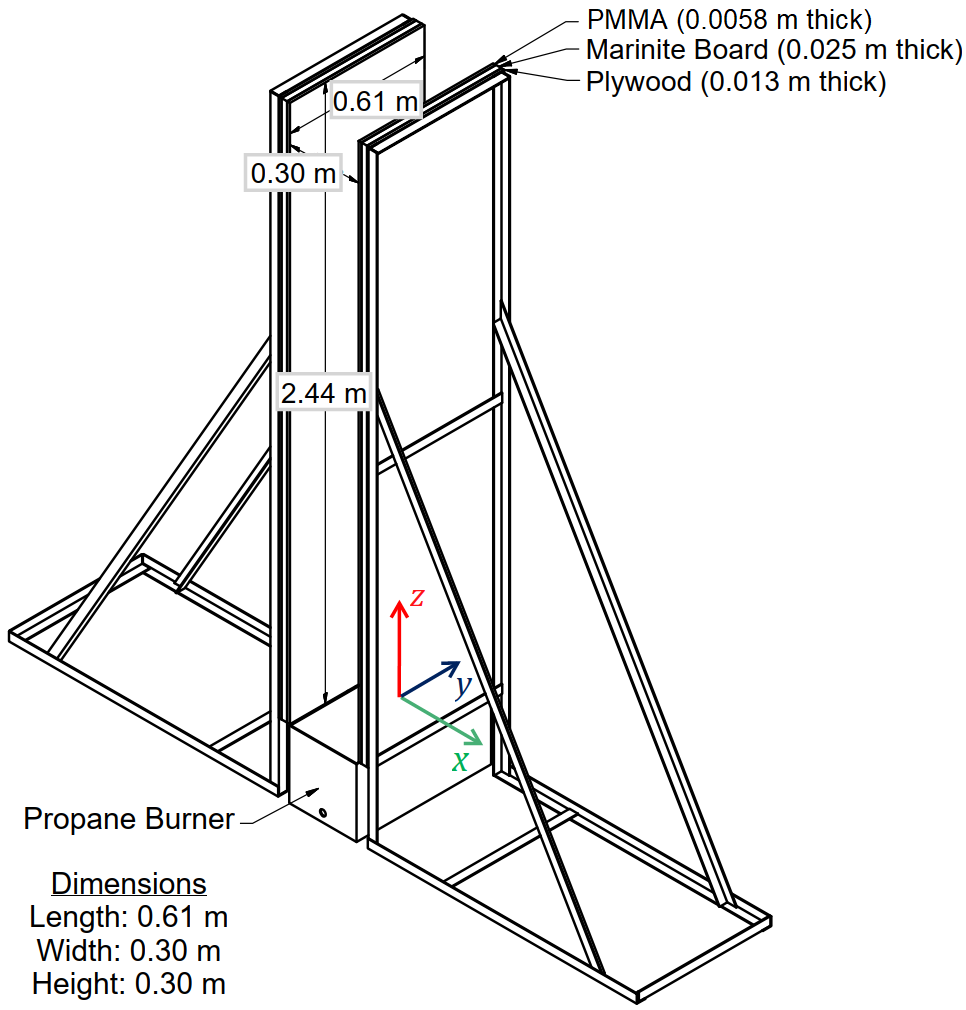
\includegraphics[width=0.75\textwidth]{{../../Fire_Growth/NIST_Parallel_Panel/Documentation/Panel_Assembly.png}}
         \caption{Schematic of the NIST Parallel Panel Apparatus}
         \label{fig:Panel_Schematic}
\end{figure}

\clearpage
\section{Communicating Results}
\subsection{How to Submit Your Results}
Experimental and Modeling Results (Fire Growth Experiments) will be submitted, stored, and made publicly available on the \href{https://github.com/MaCFP/macfp-db/Fire_Growth}{MaCFP GitHub Repository}. Details on how to contribute are available on the \href{https://github.com/MaCFP/macfp-db/wiki/How-to-Contribute}{MaCFP-db wiki}. Results can be submitted directly by creating a pull request on github or by emailing \href{mailto:randy.mcdermott@gmail.com}{Randy McDermott} or \href{mailto:isaac.leventon@gmail.com}{Isaac Leventon} directly. In either case, please ensure that your results are formatted as per the guidelines below.
%%%%%%%%%%%%%%%
**STARTER TEXT, COPIED FROM PREVIOUS GUIDELINES
For simplicity, please collect your files in a single folder with your INSTITUTE name; if emailing the data, please zip the folder to create a single attachment named “INSTITUTE.zip”. 

Note, some iteration on formatting may be required before the results can be merged into the MaCFP database.
%%%%%%%%%%%%
\subsection{File Format}
Fire growth modeling results should be organized in simple ASCII comma-delimited files (*.csv files) with clear header names in a format that matches the \href{https://github.com/MaCFP/macfp-db/tree/master/Fire_Growth}{experimental measurements} on the Github Repository. Note: For all submitted measurement data, please ensure that results are obtained with the same data acquisition rate and units. **Examples of how to format data submissions (for experimentally-measured or model-predicted results) are included below.

\textbf{Units}
This may seem like a minor issue, but we must compare the results from all groups in the same units. The units we will use are provided in the Pyrolysis Modeling section of this document. If there is ambiguity in the units or you otherwise have questions along these lines, please let us know.

\clearpage
\section{Summary}
The MaCFP-3 Workshop will be held in Tsukuba, Japan, during October 2022. This document provides guidelines for participating in this workshop. A highlight of key requests to participants is provided below.

\textbf{Gas Phase:}\\
Target xyz of certain cases? Randy/Arnaud/Anthony?**\\

\textbf{Condensed Phase:}\\
New data provided for pyrolysis model validation; request to solid-phase modelers to provided updated material property datasets (if needed) by **DATE\\
Virtual meeting to follow [**DATE + 1 month]\\

\textbf{All modelers:}
New data provided for fire growth model validation; request to gas- and solid-phase modelers to simulated key validation targets (i.e., HRR, flame to wall heat flux, and heat flux at a distance) by **DATE\\


\clearpage
\section{Contact Information}
 \subsection*{MaCFP Virtual Discussion Forum}
A Google Discussion Group for the MaCFP Working Group can be accessed here: \url{https://groups.google.com/g/macfp-discussions/}. The purpose of this forum is to facilitate data sharing and model development to improve computational predictions of thermal degradation and pyrolysis in fire.

\subsection*{Condensed Phase Phenomena Subgroup Organizing Committee}
\setlength{\parindent}{0cm}
\textbf{Benjamin Batiot} \\
Institut Pprime, France \\
    \quad\href{mailto:benjamin.batiot@univ-poitiers.fr }{benjamin.batiot@univ-poitiers.fr }
    \vspace{0.5cm}
    
\textbf{Morgan Bruns} \\
Saint Mary's University, USA\\
\href{mailto:mbruns@stmarytx.edu}{mbruns@stmarytx.edu}
    \vspace{0.5cm}

\textbf{Simo Hostikka} \\
    Aalto University, Finland\\
    \href{mailto:simo.hostikka@aalto.fi}{simo.hostikka@aalto.fi}
   \vspace{0.5cm}

\textbf{Isaac T. Leventon}\\
     National Institute of Standards and Technology, USA\\
         \href{mailto:isaac.leventon@NIST.gov }{Isaac.Leventon@NIST.gov }
   \vspace{0.5cm}

\textbf{Yuji Nakamura} \\
    Toyohashi University of Technology, Japan\\
    \href{mailto:yuji@me.tut.ac.jp}{yuji@me.tut.ac.jp}
   \vspace{0.5cm}

\textbf{Pedro Reszka} \\
    Universidad Adolfo Ibáñez, Chile\\
    \href{mailto:pedro.reszka@uai.cl}{pedro.reszka@uai.cl}
   \vspace{0.5cm}

\textbf{Thomas Rogaume} \\
Institut Pprime, France\\
    \href{mailto:thomas.rogaume@univ-poitiers.fr}{thomas.rogaume@univ-poitiers.fr}

    \vspace{0.5cm}   

\textbf{Stanislav Stoliarov} \\
University of Maryland, USA\\
    \href{mailto:stolia@umd.edu}{stolia@umd.edu}
    \vspace{0.4cm}
    

%\newpage
%\subsection*{Gas Phase Phenomena Subgroup Organizing Committee}
%\textbf{Alexander Brown} \\
%Sandia National Laboratories, USA \\

%\textbf{Andres Fuentes} \\ 
%(Universidad Técnica Federico Santa María, Chile)\\

%\textbf{Michael Gollner} \\ 
%(University of California, Berkeley, USA)\\

%\textbf{Anthony Hamins} \\ 
%(National Institute of Standars and Technology, USA)\\

%\textbf{John Hewson} \\ 
%(Sandia National Laboratories, USA)\\

%\textbf{Naian Liu} \\ 
%(University of Science and Technology of China, China)\\

%\textbf{Randy McDermott} \\ 
%(National Institute of Standards and Technology, USA)\\

%\textbf{Bart Merci} \\
%(Co-Chair) (Ghent University, Belgium)\\

%\textbf{Arnaud Trouvé} \\ 
%(Co-Chair) (University of Maryland, USA)\\

%\textbf{Yi Wang} \\
% (FM Global, USA)\\
 
%\textbf{Beth Weckman}\\
% (University of Waterloo, Canada)\\
 
 \clearpage
 \section{References}
 
\bibliography{{../MaCFP_References.bib}}

\end{document}
